\section{Game Development Languages}
In this section we examine the languages chosen by game developers. In order understand the decision making process undertaken when selecting a language for a project, the general problem of language choice is examined. Ray et al \cite{ray2014large} have conducted a large scale survey of programming language and the code quality of the resulting projects. The projects are categorised depending on the properties of the chosen languages and then the code quality is estimated. The authors posed four questions which serve as exploratory questions.

\begin{enumerate}
    \item \dquote{Are some languages more defect prone than others?}
    \item \dquote{Which language properties relate to defects?}
    \item \dquote{Does language defect proneness depend on domain?}
    \item \dquote{What is the relation between language \& bug category?}
\end{enumerate}


Ray et al, cautioned their readers against interpreting their findings as definitive proof that languages are superior or inferior to each other, this is mainly due to the fact that choice of language is a small factor in many cases. By examining the quality of the code and the contents of commit messages, Ray et al found the following answers.

\begin{enumerate}
    \item \dquote{Some languages have a greater association with defects than other languages, although the effect is small.}
    \item \dquote{There is a small but significant relationship between language class and defects. Functional languages have a  smaller  relationship  to  defects  than  either  procedural  or scripting languages.}
    \item \dquote{There is no general relationship between domain and language defect proneness.}
    \item \dquote{Defect  types  are  strongly  associated  with  languages; Some defect type like memory error, concurrency errors also depend on language primitives.  Language matters more for specific categories than it does for defects overall.}
\end{enumerate}

This examination, of the impact of language selection, suggests that language choice affects project quality as well as shedding light on how the project is affected. The next question is what languages are most often used in game development? To answer this question we conducted a small language survey of game, and game related, repositories on Github.

\subsection{Language Survey}
In this section we take a look at several game-related repositories on Github and the languages used. We used simple spreadsheet aggregation to compute the max, average and counts in the data.

\subsubsection{Threats to Validity}
In order to find repositories, Github was searched for repositories containing the word \squote{Game}. This means that the search also includes tools, engines and potentially other things.
A list of popular games and game-related tools was also included \cite{gitgames}, which is around 200 games and tools.
In total, the search yielded a little more than 4600 repositories.
Due to restrictions in Github's language \ac{API}, lines of code include white space and comments.

\subsubsection{Results}
From only looking at the popular games list, it was found that C++ is by far the most dominant language, with more than 3 billion lines as seen in \figureref{loc-top10}. The average number of languages used per repository is 3.11.

The Protogame repository by RedpointGames has a whopping 48 languages in use. It also contains different tools, such as a cross platform build tools, an \ac{API} for use with MonoGame and much more. Amazon's Lumberyard engine has the most code with a total of lines 358.943.117 lines of code, which is mostly found in Python files. Followed by a lot of C++.

\begin{figure}[H]
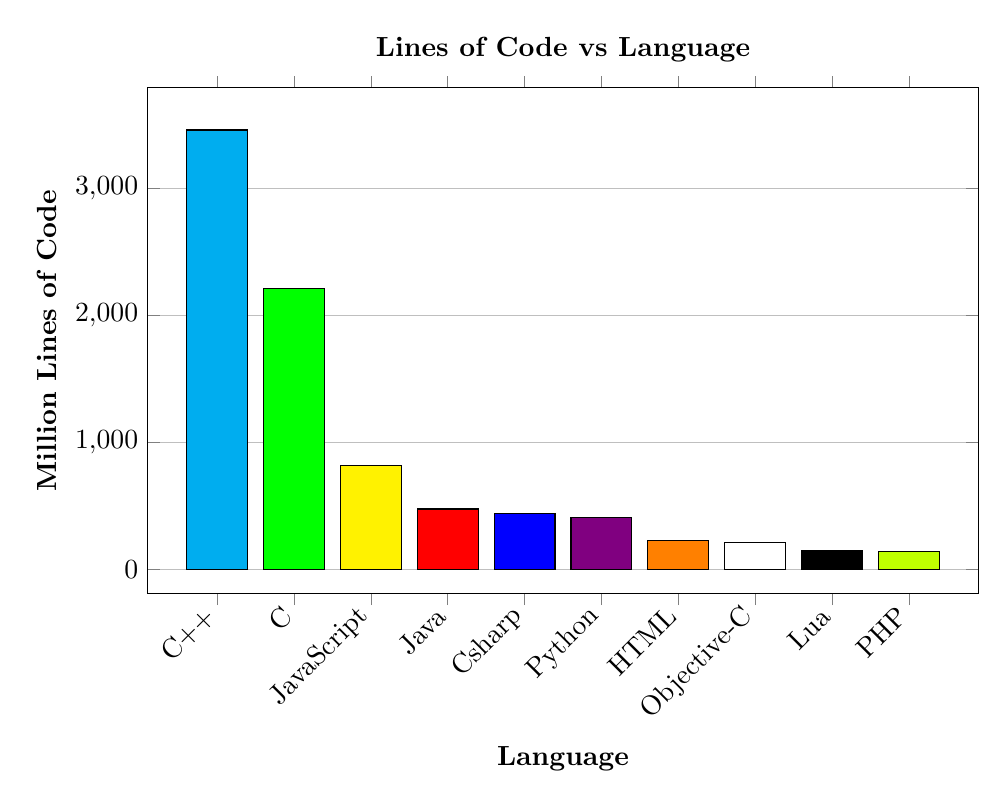
\begin{tikzpicture}
    \begin{axis}[
            title style={font=\bfseries},
            title={Lines of Code vs Language},
            label style={font=\bfseries},
            ylabel={Million Lines of Code},
            xlabel={Language},
            ybar=0pt,
            bar shift=0pt,
            width=\textwidth,
            height=8cm,
            bar width=22pt,
            ymajorgrids,
            xticklabel style={rotate=45, anchor=east},
            symbolic x coords={C++,C,JavaScript,Java,Csharp,Python, HTML,Objective-C,Lua,PHP},
        ]
        \addplot[fill=cyan]     coordinates {(C++,           3458.479714)};
        \addplot[fill=green]    coordinates {(C,             2209.641322)};
        \addplot[fill=yellow]   coordinates {(JavaScript,    817.837288)};
        \addplot[fill=red]      coordinates {(Java,          476.130697)};
        \addplot[fill=blue]     coordinates {(Csharp,        442.194502)};
        \addplot[fill=violet]   coordinates {(Python,        410.332101)};
        \addplot[fill=orange]   coordinates {(HTML,          225.246790)};
        \addplot[fill=white]    coordinates {(Objective-C,   210.542192)};
        \addplot[fill=black]    coordinates {(Lua,           149.334261)};
        \addplot[fill=lime]     coordinates {(PHP,           144.423927)};
    \end{axis}
\end{tikzpicture}
\caption{Lines of code of top 10 languages}
\label{fig:loc-top10} 
\end{figure}

